% !TEX program = xelatex

%%% Local Variables: 
%%% coding: utf-8
%%% mode: latex
%%% TeX-engine: xetex
%%% End:

\documentclass[english]{beamer}
\usepackage{mathptmx}
\usepackage[T1]{fontenc}
\usepackage{amsmath}
\usepackage{amssymb}
\usepackage{prftree, bussproofs}
\usepackage{fancyvrb}
\usepackage{soul}

\usepackage{fontspec}
\setmonofont[Scale=0.7]{FreeMono}

\newtheorem{property}[theorem]{Property}
\newtheorem{axiom}[theorem]{Axiom}

\global\long\def\evidence#1{\left\llbracket#1\right\rrbracket}
\newcommand{\form}[1]{\scalebox{1.087}{\boldmath{#1}}}
\global\long\def\ctx{\text{\ensuremath{\mathcal{\text{Ctx}}}}}%
\global\long\def\set{\text{\textbf{Set}}}%
\global\long\def\ty#1{\text{Ty}\left(#1\right)}%
\global\long\def\tm#1#2{\text{Tm}\left(#1,#2\right)}%

\newcommand{\coe}[2]{\int_{#1}{#2}}
\newcommand{\homo}[3]{\text{Hom}_{#1}\left(#2,#3\right)}
\newcommand{\type}{\mathcal{U}}
\newcommand{\pa}[3]{\texttt{Path}_{#1}\left(#2, #3\right)}
\newcommand{\compt}[5]{\texttt{comp}^{#1} \ {#2} \ \left[{#3} \mapsto{#4} \right] \ {#5}}
\newcommand{\fillt}[5]{\texttt{fill}^{#1} \ {#2} \ \left[{#3} \mapsto{#5} \right] \ {#5}}

\newcommand{\isequiv}[3]{\texttt{isEquiv} \ #1 \ #2 \ #3}

\usepackage{graphicx}

\newcommand{\fig}[2]{
    \begin{figure}\begin{center}\includegraphics[width=0.6\textwidth,height=0.6\textheight,keepaspectratio=true]{figures/#1}\caption{#2\label{#1}}\end{center}
    \end{figure}}

\newcommand{\tcol}[2]{
    \begin{columns}
        \column{.5\textwidth}
        #1
        \column{.5\textwidth}
        #2
    \end{columns}
}

\usepackage{tikz,tikz-cd}
\usepackage{tkz-graph}
\usetikzlibrary{decorations.markings,calc}
\usetikzlibrary{shapes.geometric}

\GraphInit[vstyle = Classic]
\tikzset{
LabelStyle/.style = { %rectangle, %draw,
                        minimum width = 2em, %fill = white!50,
                        text = black, font = \bfseries },
  VertexStyle/.append style = { shape = circle,
  								fill = black,
  								minimum size = 2pt,
  								inner sep=2pt,
                                %font = \Large\bfseries
                                	},
  EdgeStyle/.append style = {->, bend left} }


\pgfdeclarelayer{edgelayer}
\pgfdeclarelayer{nodelayer}
\pgfsetlayers{edgelayer,nodelayer,main}

\tikzstyle{none}=[inner sep=0pt]


\tikzstyle{simple}=[-,draw=black,line width=1.000]
\tikzstyle{arrow}=[-,draw=black,postaction={decorate},decoration={markings,mark=at position 0.5 with {\arrow{>}}}]

\usepackage{graphicx}
\usepackage{multimedia}

\makeatletter

%%%%%%%%%%%%%%%%%%%%%%%%%%%%%% LyX specific LaTeX commands.
%% Because html converters don't know tabularnewline
\providecommand{\tabularnewline}{\\}

%%%%%%%%%%%%%%%%%%%%%%%%%%%%%% Textclass specific LaTeX commands.
% this default might be overridden by plain title style
\newcommand\makebeamertitle{\frame{\maketitle}}%
% (ERT) argument for the TOC 
\AtBeginDocument{%
  \let\origtableofcontents=\tableofcontents
  \def\tableofcontents{\@ifnextchar[{\origtableofcontents}{\gobbletableofcontents}]}
  \def\gobbletableofcontents#1{\origtableofcontents}
}

%%%%%%%%%%%%%%%%%%%%%%%%%%%%%% User specified LaTeX commands.
\usetheme{default}
% or ...dff

\setbeamercovered{transparent}
% or whatever (possibly just delete it)


\addtobeamertemplate{navigation symbols}{}{%
    \usebeamerfont{footline}%
    \usebeamercolor[fg]{footline}%
    \hspace{1em}%
    \insertframenumber/\inserttotalframenumber{}
}

\makeatother

\usepackage{babel}
\begin{document}
\title[Cubical models for Univalence]{The Constructive Model of \\ Univalence in  Cubical Sets}
\subtitle{Literature review}
\author[W. Vanhulle]{W. Vanhulle\inst{1} \and A. Nuyts\inst{2}\and D. Devriese\inst{3}}
\institute[KUL]{\inst{1}Student \and \inst{2}Supervisor \and \inst{3}Promoter}
\date[30/05/19]{45 min. public seminar}

\makebeamertitle

\pgfdeclareimage[height=0.5cm]{institution-logo}{figures/kuleuven}
\logo{\pgfuseimage{institution-logo}}

\AtBeginSubsection[]{%
  \frame<beamer>{ 
    \frametitle{Outline}   
    \tableofcontents[currentsection,currentsubsection] 
  }
}

%\beamerdefaultoverlayspecification{<+->}
\begin{frame}{Outline}

\tableofcontents{}

\end{frame}

\section{Introduction}

\begin{frame}{}
    \setbeamercovered{invisible}
    A mathematician is asked by a friend who is a devout Christian: ``Do you believe in one God?'' 
    \begin{quotation}
    What does he reply?
    \end{quotation}
    \pause{}
    
    
    He answers: ``Yes -- up to isomorphism.'' (© Michael Benjamin Stepp)

\fig{isomorphism}{Monkeys looking at isomorphic monkeys.}
\end{frame}


\begin{frame}{Algebraic Topology}

Isomorphism in algebraic topology is ``homotopy equivalence''

\begin{columns}
    \column{.5\textwidth}
    \fig{mug}{A mug}
    \column{.5\textwidth}
    \fig{donut.jpg}{A donut}
\end{columns}

homotopy equivalent spaces have the same ``number of \(n\)-dimensional holes''

\end{frame}


\begin{frame}{Holes are homotopy groups}

computed by looking at homotopy classes of embeddings \[S^n \rightarrow X, \quad \text{or } {[0,1]}^n \rightarrow X\]

\tcol{
                \fig{loops}{A donut has two 1-dimensional homotopy classes.}
}
    {
                \fig{basketball_hollow}{A ball without center has two 2-dimensional homotopy classes.}
}
\end{frame}


\begin{frame}{Type theory}
    
    Two meanings/subfields:
    \begin{itemize}
        \item verifying computation in programming languages
        \begin{figure}
            \input{figures/haskell.verbatim}
            \caption{A typed recursive function in Haskell}
        \end{figure}
    
        \pause{}
        \item alternative constructive foundation of mathematics
        \begin{figure}
            \input{figures/agda_comp.verbatim}
            \caption{Definition of the topological space \(S^1\) in Agda}
        \end{figure}
    
    \end{itemize}

    
\end{frame}

\begin{frame}{Type theory as foundation of mathematics}{Russel, 1907}

Invented to prevent paradox:


    $$ R = \{x \mid x \not \in x \}, R\in R \Leftrightarrow \not \in R $$
    

Solution was:
\begin{itemize}
\item replace sets (and propositions) by types and elements by terms, $$x \in R \Rightarrow x : R$$
\item types belong to universe hierarchy 
        \[\exists i, R : \mathcal{U}_i, \quad \mathcal{U}_0 : \mathcal{U}_1 : \ldots \]
\item constructive logic and formation rules
\end{itemize}

\begin{quotation}
$x \not \in x$ is not a valid proposition anymore
\end{quotation}

\end{frame}

\begin{frame}{equality type}{Martin-L\"of, 1984}
    
    Leibniz's principle (axiom):
         \[f = g \Leftrightarrow f(x) = g(x), \forall x\]
    
    Not an axiom in type theory for decidability reasons.
    
    \pause
    Equality ``\(=\)'' added as a type called \emph{propositional equality}:

    \begin{itemize}
        \item weaker than equality ``by definition''.
        \item stronger than equivalence.
    \end{itemize}

\end{frame}

\begin{frame}{Identity eliminator}{Martin-L\"of, 1984}

       Elimination rule of equality type:

    \begin{definition}[path induction]
            Given the following terms:
        \begin{itemize}
            \item a predicate \(C : \prod_{x,y:A} (x =_A y) \rightarrow \mathcal{U}\)
            \item the base step \(c:\prod_{x:A} C(x,x,\texttt{refl}_x)\)
        \end{itemize}
            there is a function \(f: \prod_{x,y:A} \prod_{p:x=_Ay}C(x,y,p)\) such that \(f(x,x,\texttt{refl}_x) \equiv c(x)\).
        
    \end{definition}

    \pause

    (describes how to compute with the equality type)
    
\end{frame}

\begin{frame}{Intuition identity eliminator}

    Role of eliminator:
    \begin{quotation}
        To prove a property \(C\) that depends on terms $x,y$ and equalities $p:x=y$  it suffices to consider all the cases where
        
        \begin{itemize}
            \item $x$ is definitionally equal to $y$
            \item the term of the intensional equality type under consideration is $\texttt{refl}_x : x = x$.
        \end{itemize}
        \end{quotation}

        Implications:
        \begin{itemize}
            \item proves transitivity, symmetry
            \item equality type can have multiple terms
        \end{itemize}

\end{frame}


\begin{frame}{Homotopy type theory (HoTT)}{Awodey, 2006}

Gives \emph{homotopy} interpretation to equality type:

%\includegraphics[width=0.8\textwidth]{figures/}
\centering
$$ p,q : a =_X b \quad r,s : p =_{\texttt{Id}_X(a,b)} q$$ 

\begin{tikzpicture}
  [decoration={markings,mark=at position 0.5 with {\arrow{>}}},
   witharrow/.style={postaction={decorate}},
   dot/.style={draw,fill,circle,inner sep=1.5pt,minimum width=0pt}
  ]

  % rectangle 1
  \begin{scope}
     \draw[thick]
       (0,0) coordinate (a1) -- node[left]     {$a$} (0,2) coordinate (d1)
       (2,0) coordinate (b1) -- node[right](q1){$b$} (2,2) coordinate (c1);
     \draw[xstep=2,ystep=1/3] (a1) grid (c1);
     \draw[thick,witharrow] (d1) -- node[above]    {$p$}(c1);
     \draw[thick,witharrow] (a1) -- node[below](f1){$q$}(b1);
  \end{scope}
  
  
  \begin{scope}[shift={(6,0.5)}]
    \node[dot,label={[left] $a$}] (a3) at (0,0) {};
    \node[dot,label={[right]$b$}] (b3) at (4,0) {};
    \draw[thick,witharrow] (a3) to[out=50,in=150]node[above]{$p$} (b3);
    \foreach \o/\i in {40/160,30/170,20/180,10/190,-10/200}
       \draw (a3) to[out=\o,in=\i]  (b3);
    \draw[thick,witharrow] (a3) to[out=-20,in=-130]node[below]{$q$} (b3);
    \draw ($0.5*(a3)+0.5*(b3)$) circle[x radius=2.5,y radius=1.5];
    \node at ($(a3)+(0.5,0.8)$) (X3) {$X$};
    \node at ($(a3)+(0.5,-0.8)$) (X4) {};
  \end{scope}

%connections
  \draw[-stealth,shorten >=4mm] (q1) to[out=30,in=150]node[above]{$r$} (X3);
  \draw[-stealth,shorten >=4mm] (q1) to[out=-30,in=-150]node[below]{$s$} (X4);
\end{tikzpicture} 



$\Rightarrow$ alternative foundations for mathematics based on type theory and topology

\end{frame}

% \begin{frame}{Short history of HoTT }

% \begin{itemize}
%  \item groupoid model, Hofmann  (1996)
%  \item univalence axiom, Voevodsky (2009)
%  \item univalent foundations, Voevodsky, Grayson, Coquand (2013)
% \end{itemize}

% \begin{figure}[h!]
% \centering    
% 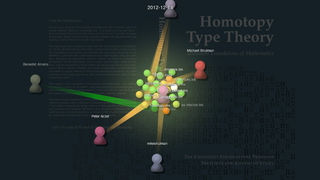
\includegraphics[width=0.7\textwidth]{figures/HoTT-pic.png}
%   \caption{Univalent foundations 2013--2014}
%  \end{figure} 


% \end{frame}

\begin{frame}{Role of univalence}{Voevodsky, 2009}

\begin{axiom}[Univalence axiom] 
 Given types $X,Y : \mathcal{U}$ for some universe $\mathcal{U}$, the map \(\Phi_{X,Y}: (X=Y) \rightarrow (X \simeq Y)\) is an equivalence of types. 
\end{axiom}

\begin{itemize}
    \item equivalence of types is a bijection for set-like types \[\mathbb{N} \simeq \mathbb{N}_0 \]
    \item univalence implies \[\mathbb{N} \simeq \mathbb{N}_0 \Rightarrow \mathbb{N} = \mathbb{N}\]

    \item forces multiple terms of equality
\end{itemize}

\pause
\begin{quotation}
$\Rightarrow$ terms of equality are like paths
\end{quotation}

% \begin{figure}[h!]
% \centering    
% 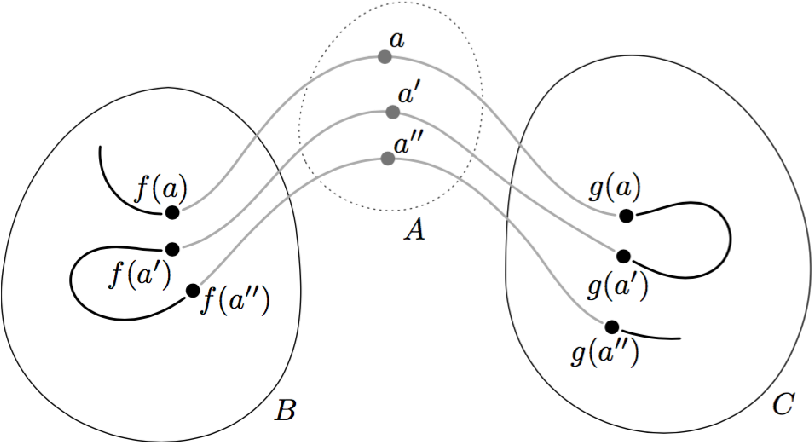
\includegraphics[width=0.5\textwidth]{figures/seifert.png}
%   \caption{Seifert-Van Kampen theorem in HoTT. Hou, Shulman (2016)}
%  \end{figure} 


\end{frame}

\begin{frame}[fragile]
    \frametitle{Consequences of path interpretation}
     
     
     \tcol{

        in general:
        \begin{itemize}
          \item equivalence behaves like homotopy equivalence
            \item mathematics ``up to homotopy''
            \item lifting of path $p$ as in  algebraic topology: \emph{transport} gives the other ending point of $p_\star$
        \end{itemize}
     }
     {
        \fig{cover}{Jeff Erickson, 2009}
     }     
\end{frame}
    


\begin{frame}{Origin univalence}{Grayson, 2018}

\begin{columns}[c]
    \column{.5\textwidth}
        \begin{center}
            \begin{figure}[h!]
                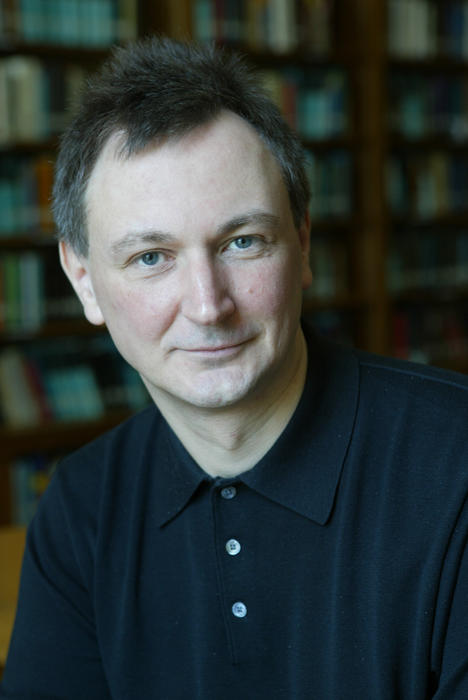
\includegraphics[height=.7\textheight]{figures/voevodsky.jpg}
                \caption{Vladimir Voevodsky (1966 - 2017)}
            \end{figure} 
        \end{center}
    \column{.5\textwidth}

            Why is it called ``univalent''?


        \pause

        \begin{quotation}
        ... these foundations seem to be faithful to the way in which I think about mathematical objects in my head ...
        \end{quotation}

        faithful = univalent in a Russion translation of Boardman (2006)

\end{columns}
\end{frame}



\begin{frame}{Computing with univalence}{Huber, 2015}

What about:
\begin{itemize}
\item implementing HoTT?
\item calculations with very simple types as $\mathbb{N}$?
\end{itemize}

\begin{quotation}
Can we, given a term $t: \mathbb{N}$ constructed using the univalence axiom, construct two terms $u : \mathbb{N}$ and $p : t =_{\mathbb{N}} u$ such that $u$ does not involve the univalence axiom?
\end{quotation}

\pause

 $\Rightarrow$ canonicity of $\mathbb{N}$ in cubical type theory (CTT)

$$ t \equiv ua ( ... )  \rightsquigarrow u \equiv S ( \dots ( 0 ) \ldots ) : \mathbb{N}  $$


\end{frame}




\section{Cubical model}

\begin{frame}{Cubical type theory}{Cohen et al., 2015}

A constructive extension of HoTT with dimension variables $i,j,k : \mathbb{I}$ (cubes) as primitives:

\begin{figure}[h!]
    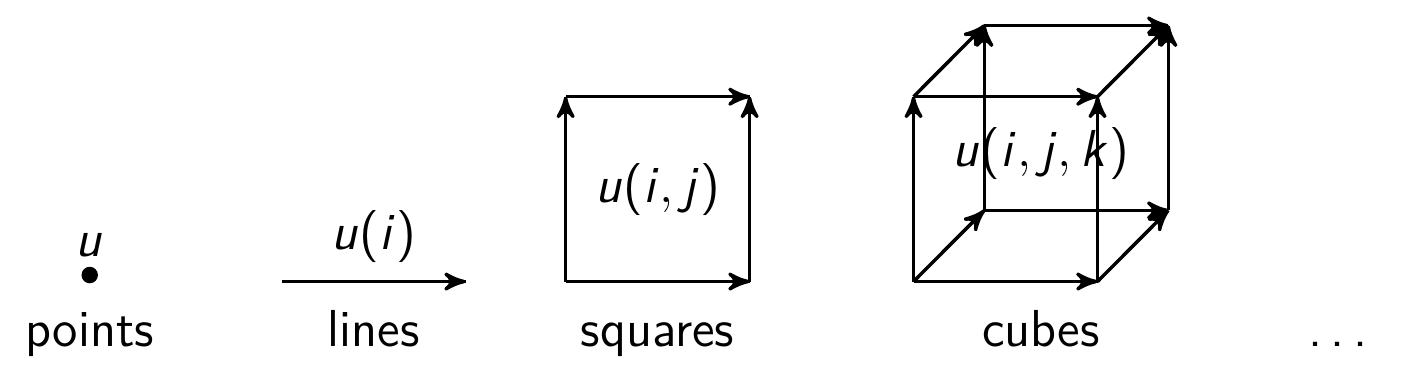
\includegraphics[width=.7\textwidth]{figures/cubes.png}
    \caption{Discrete ``$n$-cubes''. Huber (2016)}
\end{figure}


\begin{itemize}
\item univalence becomes \emph{constructable}
\item computational interpretation for univalence 
\end{itemize}

\end{frame}


\begin{frame}{Are cubes a good idea?}{EnigmaChord, 2016}

\fig{cube-joke.jpg}{}

\pause

(yes, they model n-dimensional homotopies)

\end{frame}


\begin{frame}{Cubes model homotopy}{Altenkirch, Brunerie, Licata, et. al 2013}
 
Homotopy groups are defined as equivalence classes:
$$[0,1]^n \rightarrow X$$

In homotopy type theory:
\begin{quotation}
 higher-dimensional paths $\cong$ higher-dimensional eqalities.
\end{quotation}
\pause

Cubes give discrete description of higher-dimensional paths:
\begin{itemize}
 \item equalities $\Rightarrow$ edges of cubes
 \item equalities between equalities (homotopies) $\Rightarrow$ faces of cubes, ...
\end{itemize}

% \begin{figure}
%  \begin{tikzpicture} [decoration={markings,mark=at position 0.5 with {\arrow{>}}},
   witharrow/.style={postaction={decorate}},
   dot/.style={draw,fill,circle,inner sep=1.5pt,minimum width=0pt}
  ]
		\begin{pgfonlayer}{nodelayer}
		\node [style=none] (0) at (0, -0) {};
		\node [style=none] (1) at (3, -0) {};
		\node [style=none] (2) at (0, 3) {};
		\node [style=none] (3) at (3, 3) {};
		\node [style=none] (4) at (1, 2) {};
		\node [style=none] (5) at (2, 1) {};
		\node [style=none] (6) at (2, 0) {};
		\node [style=none] (7) at (0, 2) {};
		\node [style=none] (8) at (0, 3) {};
		\node [style=none] (9) at (1, 3) {};
		\node [style=none] (10) at (1, 3) {};
		\node [style=none] (11) at (2, 3) {};
		\node [style=none] (12) at (2, 3) {};
		\node [style=none] (13) at (-2, -1) {};
		\node [style=none] (14) at (1, -1) {};
		\node [style=none] (15) at (-4, -0) {};
		\node [style=none] (16) at (-1, -0) {};
		\node [style=none] (17) at (-4, 3) {};
		\node [style=none] (18) at (0.75, -0) {};
		\node [style=none] (19) at (3, 2) {};
		\node [style=none] (20) at (3, 0.75) {};
		\node [style=none] (21) at (0, 1) {};
	\end{pgfonlayer}
	\begin{pgfonlayer}{edgelayer}
		\draw [style=simple] (0.center) to node[left]{$\texttt{P\ 0\ j}$} (2.center);
		\draw [style=arrow] (0.center) to node[above]{$\texttt{P\ i\ 0}$} (1.center);
		\draw [style=simple] (2.center) to node[above]{$\texttt{P\ i\ 1}$} (3.center);
		\draw [style=arrow] (3.center) to node[right]{$\texttt{P\ 1\ j}$} (1.center);
		\draw [style=arrow] (2.center) to node[below]{$\texttt{P}$} (1.center);
		\draw [style=arrow] (13.center) to node[below]{$\texttt{A\ i}$} (14.center);
		\draw [style=arrow] (15.center) to node[left]{\texttt{j}} (17.center);
		\draw [style=arrow] (15.center) to node[below]{\texttt{i}} (16.center);
		\draw [style=arrow] (7.center) to (4.center);
		\draw [style=arrow] (9.center) to (4.center);
		\draw [style=arrow] (11.center) to (5.center);
		\draw [style=arrow] (21.center) to (5.center);
	\end{pgfonlayer}
\end{tikzpicture} 

%  \caption{ \texttt{P} is an equality (homotopy) between equality $A\ i$ and constant equality at $A \ 0$}
% \end{figure}
\end{frame}

\begin{frame}{Operations on cubes}{Bezem, Coquand, Huber et al., 2013}
 
\begin{columns}[c]
    \column{.5\textwidth}
        \begin{center}
            \begin{figure}[h!]
                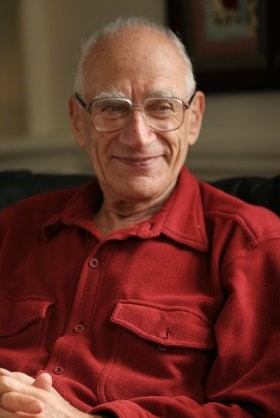
\includegraphics[height=.6\textheight]{figures/kan.jpg}
                \caption{Daniel Kan (1927 --- 2013)}
            \end{figure} 
        \end{center}
    \column{.5\textwidth}
        
        Necessary for modelling HoTT:
        
        \begin{itemize}
         \item  composition $\Rightarrow$ equality type
         \item glueing $\Rightarrow$ univalence
        \end{itemize}


        \begin{figure}[h!]
                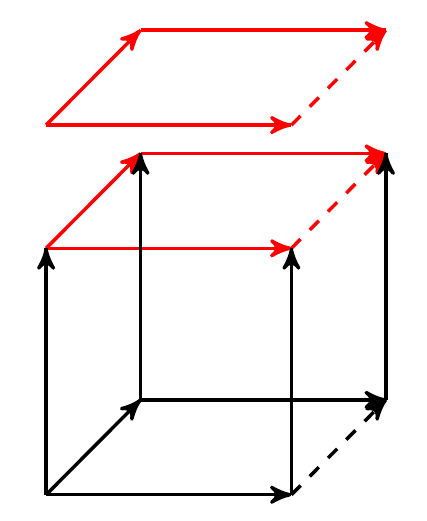
\includegraphics[height=.4\textheight]{figures/extension.png}
        \end{figure} 

        
\end{columns}
\end{frame}



\begin{frame}{Presheaves on $\mathcal{C}$}{Hofstra, 2014}
 
 Maps (contravariant functors) $\mathcal{C} \rightarrow \mathbf{Set}$ denoted by $\hat{\mathcal{C}}$
 
 \begin{itemize}
 \item generalize sheaves (see sheafication)
 \item model type theories, Dybjer (1994)
 \end{itemize}
 
 \begin{example}[Reflexive directed graphs]    
 Take $\mathcal{C} = \{0,1\}$ and $\text{Hom}_{\mathcal{C}}= \{B,E,R\}$
 
  
\begin{tikzpicture}
  %\SetGraphUnit{5}
  \Vertex[x=0, y=0]{A}
  \Vertex[ x=2,y=0]{B}
  \Edge[](A)(B)
  
  \Vertex[x = 3, y = -1]{C}
  \Vertex[x = 4, y = 1]{D}  
  \Edge[](C)(D)
  \Vertex[x = 5, y = -1]{E}
  \Edge [](C)(E)
  
  \Loop[dist = 1cm, dir = NO](B)
  \Loop[dist = 1cm, dir = NO](A)
  \Loop[dist = 1cm, dir = NO](C)
  \Loop[dist = 0.5cm, dir = NO](D)
  \Loop[dist = 1cm, dir = NO](E)
\end{tikzpicture} 
    
 
 
 
\end{example} 

 
\end{frame}

\begin{frame}{Presheaf model on $\mathcal{C}$}{Dybjer, 1994}
 
 Gives interpretations for stuff in type theory:
 \begin{itemize}
  \item contexts $\Gamma$ are the category $\widehat{\mathcal{C}}$
  \item types are a presheaf $$\widehat{\int_{\mathcal{C}} \Gamma}$$
  \item terms are elements of $$\prod _{I \in \mathcal{C}, \rho \in \Gamma (I)} A(I,\rho)$$
 \end{itemize}

 \pause
 
 Bonuses:
 
 \begin{itemize}
  \item verify consistency of type theory in sets
  \item find primitives for implementations
 \end{itemize}
 
\end{frame}

\begin{frame}{Types with presheaves}

  \begin{example}
  A type $A$  over $\mathcal{C} = \{0,1\}$ is a refined graphs,   
  terms $a,b:A$ are edges in refined graph:
  \begin{figure}\label{depgraphdiag}
\begin{center} 
\begin{tikzpicture}
  %\SetGraphUnit{5}
  \Vertex[L = $\rho B$, x=0, y=0]{A}
  \Vertex[L = $\rho E$, x=4,y=0]{B}
  \Edge[label = $\rho$](A)(B)
  \Vertex[L = $(a\rho) B$, x = 0, y = 2]{C}
  \Vertex[L = $(a\rho) E$, x = 4, y = 4]{D}
  
  \Edge[label = $a \rho$](C)(D)
  \Vertex[L = $ (b\rho) E$, x = 4, y =2]{E}
  \Edge [label = $ b \rho$](C)(E)
  \Loop[dist = 1cm, dir = NO, label = $R$, labelstyle=left](C)
  \Loop[dist = 1cm, dir = NO, label = $R$, labelstyle=left](A)
\end{tikzpicture} 

%%\begin{tikzpicture}
%%  %\SetGraphUnit{5}
%%  \Vertex[L = $\rho E$, x=0, y=0]{A}
%%  \Vertex[L = $\rho B$, x=4,y=0]{B}
%%  \Edge[label = $\rho$](A)(B)
%%  \Vertex[L = $(a\rho) E$, x = 0, y = 2]{C}
%%  \Vertex[L = $(a\rho) B$, x = 4, y = 4]{D}
%%  
%%  \Edge[label = $a \rho$](C)(D)
%%  \Vertex[L = $ (b\rho) B$, x = 4, y =2]{E}
%%  \Edge [label = $ b \rho $](C)(E)
%%  \Loop[dist = 3cm, dir = NO, label = $(a\nu)R$](C)
%%  \Loop[dist = 3cm, dir = NO, label = $\nu R$](A)
%%\end{tikzpicture} 
%%
  
\end{center}    
  \end{figure}
 \end{example}
\end{frame}

\begin{frame}{Distributive lattice}
 
%  In cubical type theory, $\mathcal{C} \not = \{0, 1\}$ but $\mathcal{C} = \square$.
%  
%  \pause 
%  

 
 
  \begin{columns}[c]
    \column{.5\textwidth}
          Let $i, j , k, ... \in \mathbb{A}$ countable = ``dimension variables'' 
 
 \begin{definition}[Free De Morgan algebra]
 Distributive lattice containing:
 
 \begin{itemize}
  \item $i \wedge j$ (min of $i$, $j$)
  \item $i \vee 0$ (computes to $i$)
  \item $\neg k$ (negation)
  \item de Morgan rules.
 
 \end{itemize}

 ... denoted by $dM(i,j,k,...)$
\end{definition}
 

    \column{.5\textwidth}
        \begin{figure}
       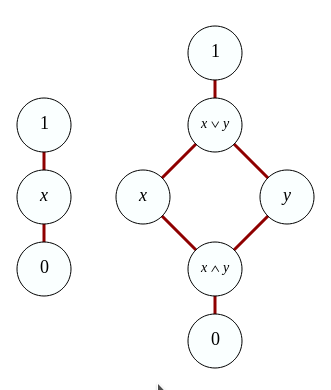
\includegraphics[width=0.8\textwidth]{figures/lattice}
       \caption{A distributive lattice}
       \end{figure}
\end{columns}
 
 
\end{frame}

\begin{frame}
 


 
 \begin{definition}[cube category $\square$]
 
  objects are $\{ I \mid |I| < \infty , I \subset \mathbb{A} \}$
  morphisms $J\rightarrow I$ are maps $I \mapsto dM(J)$ 
%\item types float above contexts
 
 \end{definition}
 
  \begin{example}[presheaf model on $\square$]
 contexts $\Gamma$ are presheaves $\square \rightarrow \mathbf{Set}$
 shaped by lattice structure $\Rightarrow$ complicated!
 
 \begin{figure}
 
 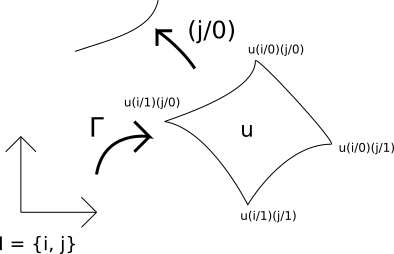
\includegraphics[width=0.6\textwidth]{figures/context}
 
  \caption{a context $\Gamma$ applied to $\{i,j\}$}
  \end{figure}
 \end{example}
 
\end{frame}

\begin{frame}{Types in $\widehat{\square}$}
 \begin{figure}
\centering
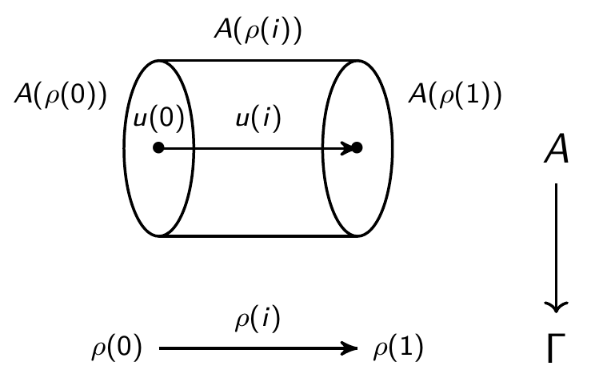
\includegraphics[width=0.7\textwidth]{figures/types}
\caption{A type $A$ within context $\Gamma$. Huber (2016)}
 \end{figure}
 
\end{frame}


\begin{frame}{Types in presheaf models}

In the presheaf model on $\square$:
\begin{itemize}
    \item types more complicated
    \item types no longer simply nested graphs
\end{itemize}


\begin{lemma}[Characterization of types]

If $\Gamma \in \widehat{\mathcal{C}}$, then 
$$\text{Ty}(\Gamma) \cong \left\{ (\Delta, \sigma) \mid \Delta \in \widehat{\mathcal{C}}, \sigma \in \text{Hom}_{\text{Ctx}}(\Delta , \Gamma) \right\}$$
\end{lemma}

\pause


Interpreting types in presheaf model $\square$ hard but possible! 



\end{frame}

\begin{frame}{Path type}{Bezem, Coquand, 2013}
 
 Syntactical definition of \texttt{Path} type with typing rules:

\begin{prooftree}
\AxiomC{$ i : \mathbb{I} \vdash t : A$}
\AxiomC{$i : \mathbb{I} \vdash t(i/0) = a : A$}
\AxiomC{$i : \mathbb{I} \vdash t(i/1) = b : A$}
\TrinaryInfC{$() \vdash \left< i \right> t : \texttt{Path} \ a\   b$}

\end{prooftree}

% \begin{prooftree}
% \AxiomC{$\Gamma \vdash t : \pa{A}{u_0}{u_1}$}
% \UnaryInfC{$\Gamma \vdash t 0 = u_0 : A$}
% \end{prooftree}
% 
% \begin{prooftree}
% \AxiomC{$\Gamma \vdash t : \pa{A}{u_0}{u_1}$}
% \UnaryInfC{$\Gamma \vdash t 1 = u_1 : A$}
% \end{prooftree}

\begin{itemize}
 \item almost models equality type
 \item not necessarily transitive $\Rightarrow$ composition operation
\end{itemize}


\begin{figure}
\centering
\[ \begin{tikzcd}
a \arrow[r, dashrightarrow] 
& c  \\
a 	\arrow[u, "refl"]	
	\arrow[r, "p \  i"]
& b  \arrow[u, "q \ j"] 
\end{tikzcd}
\] 

\caption{Transitivity can be proven with composition operation.}
\end{figure}

\end{frame}

\begin{frame}{Constructive model of type theory}{}
 


 \begin{columns}[c]
    \column{.5\textwidth}
         Other types can be interpreted in the presheaf model  $\widehat{\square}$
          for constructive model for type theory:
 \begin{itemize}
  \item product, sum types
  \item natural numbers
 \end{itemize}
 
        Univalence proven with:
        
       \begin{itemize}
        \item concepts from simplicial set model (Streicher, Voevodsky, Kapulkin et al. 2006 -- 2012)
        \item partial types and glueing construction 
       \end{itemize}
    \column{.5\textwidth}
        \begin{figure}
       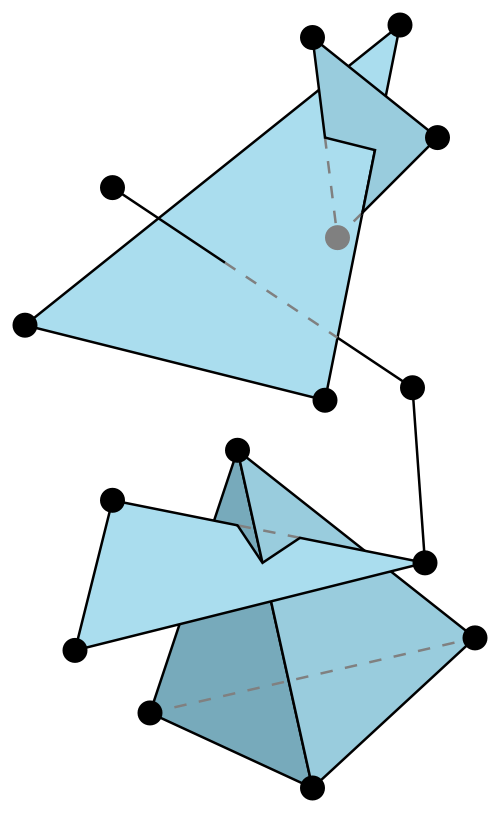
\includegraphics[width=0.7\textwidth]{figures/simplex}
       \caption{Related concept of a simplicial complex}
       \end{figure}
\end{columns}
 
\end{frame}

\begin{frame}{Partial types} 
 Partial types are only defined on subpolyhedra of cubes:
 
 
 \begin{figure}
    \centering
  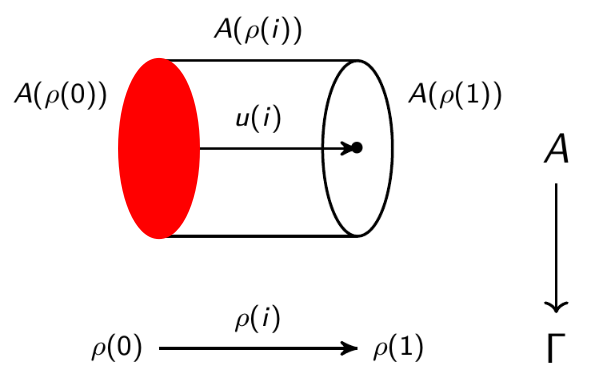
\includegraphics[width=0.7\textwidth]{figures/types_side}
  \caption{The partial type $A(i/0)$ in type $A$, syntactically: $A\ [(i = 0) \mapsto A(i/0)]$.}
 \end{figure}

 
 
\end{frame}

\begin{frame}{Glueing equivalences}
  
  Equivalences are a crucial ingredient for the univalence axiom:
  \begin{itemize}
   \item maps $f : T \rightarrow A$ that correspond to homotopy equivalences
   \item have inverse up-to some paths
  \end{itemize}

  
   The \texttt{Glue} type was introduced to prove univalence:
   \begin{itemize}
    \item very complicated typing rules
    \item glue equivalences  over partial types together:
   \end{itemize}

 
\begin{figure}
 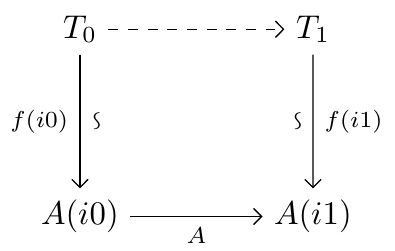
\includegraphics[width=0.5\textwidth]{figures/glue}
% \caption{Glueing the equivalence over the partial type $T$.}
\end{figure}

  
 
\end{frame}

\begin{frame}{Proving univalence}{Cohen, Coquand, Huber, Moertberg (2015)}

\begin{axiom}[Univalence axiom]
 Given types $X,Y : \mathcal{U}$ for some universe $\mathcal{U}$, the map $\Phi_{X,Y}: (X=Y) \rightarrow (X \simeq Y)$ is an equivalence of types. 
\end{axiom}


 

\begin{proof}

\begin{itemize}

\item The existence of a map $\texttt{ua} : (X\simeq Y) \rightarrow (X = Y)$ proven with \texttt{Glue} construction:
 
 
 $$i : \mathbb{I} \vdash E= \texttt{Glue} \left[ (i=0) \mapsto (X, f),(i=1) \mapsto\left(Y, \texttt{id}_{Y}\right) \right] Y$$
 
 $E$ is a path (equality) from $X$ to $Y$.
 
 \item Remainder proven with ``contractibility of singletons''.
 
 \end{itemize}
\end{proof} 

\end{frame}


\section{Applications}


\begin{frame}{Applying \texttt{ua} from univalence }
 
 \begin{example}[Monoids]
 
 $$M_1  \equiv (\mathbb{N}, (m,n)\mapsto m+n, 0)$$ and $$M_2 \equiv (\mathbb{N}_0, (m,n)\mapsto m+n -1, 1)$$
\begin{itemize}
 \item  are isomorphic by $$\lambda n \rightarrow n + 1 $$ 
 \item (path-) equal in CTT
\end{itemize}
 
 \end{example}
 

 
\end{frame}

\begin{frame}[fragile]
\frametitle{Definition of a \st{monoid} magma}
%{Building a path}

setoid encoding uses operator ``\texttt{∙}'' and equivalence ``\texttt{≈}'':

\begin{figure}
\begin{BVerbatim}
notZero n = Σ ℕ (λ m → (n ≡ (suc m)))
ℕ₀ = Σ ℕ (λ n → notZero n) 

op₂ : Op₂ ℕ₀
op₂ (x , p)  (y , q) = 
    (predℕ (x + y) , (predℕ (predℕ (x + y)) , sumLem x y p q) )

M₂ : Algebra.Magma _ _
M₂ = record { 
  Carrier = ℕ₀ ;
  _≈_ = (_≡_) ;
  _∙_ = op₂ ;
  isMagma = ... ,
  }
\end{BVerbatim}
\end{figure}
 
\end{frame}

\begin{frame}[fragile]
\frametitle{Equality of carrier sets}

 $\mathbb{N} \rightarrow \mathbb{N}_0: n\mapsto n + 1 $ is bijection
 
 \begin{itemize}
  \item is equivalence of (set-like) types
  \item univalence/\texttt{ua} returns equality \texttt{ℕ ≡ ℕ₀}
 \end{itemize}
 
 
 \begin{figure}
 \begin{BVerbatim}
f : ℕ → ℕ₀ 
f n = (suc n , ( n , refl ) )
...
fEquiv : ℕ ≃ ℕ₀ 
fEquiv = (f ,  isoToIsEquiv (iso f g l' r'))

fEq : ℕ ≡ ℕ₀ 
fEq i = ua fEquiv i
 \end{BVerbatim}
\end{figure}

\end{frame}





\begin{frame}[fragile]
\frametitle{Equality of \st{monoids} magmas}

Defined for every component of record type:

\begin{figure}
\begin{BVerbatim}
mPath : s₁ ≡ s₂
mPath = λ i → record {
   Carrier = (fEq i) ;
   _≈_ =  _≡_;
   _∙_ = transOp' i ;
   isMagma = record {
    isEquivalence = ≡equiv  ;
     ∙-cong   = ?
     }
   }
\end{BVerbatim}
\end{figure}

\texttt{transOp'} defined by transporting along \texttt{ℕ ≡ ℕ₀}, proofs can be transported over \texttt{s₁ ≡ s₂}.

\end{frame}

\begin{frame}{Higher homotopies of spheres}{}

    Types in HoTT and CTT are topological spaces.
    Homotopy groups compute number of higher-dimensional holes:

    \fig{groups}{Higher homotopy groups of $S^n$}
    Homotopy groups can be defined in CTT as datatypes

\end{frame}


\begin{frame}{Implementation in CTT}{Brunerie, 2016}

 \begin{columns}%[c]
    \column{.6\textwidth}
        
        \begin{theorem}
            $\pi _ 4 (S^3) \cong \mathbb{Z}_n$ for $n=2$ 

            \end{theorem}
            \begin{itemize}
            \item proven in HoTT with univalence
            \item $n$ implemented in CTT as a function
            \item canonicity predicts termination
            \end{itemize}
        (bug in Agda or CTT prevents evaluation)

        \column{.4\textwidth}
            \begin{figure}
                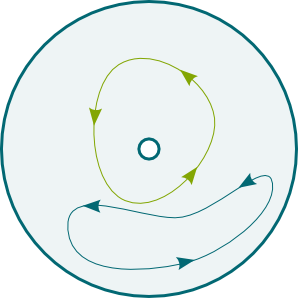
\includegraphics[height=0.4\textheight]{figures/loops}
                \caption{The case $S^1$ is simply $\mathbb{Z}$  (drawing from science4all)}
            \end{figure}
    \end{columns}

\end{frame}

\section*{Summary}


\begin{frame}{Other research}{Licata, Harper, Cavallo, Orton et al., 2018}
    \begin{itemize}
        \item computational type theory is an alternative implementation 
        \item composition operation may not be necessary
        \item alternatives to complicated glue types: fundamental axioms and language of topoi
    \end{itemize}
\end{frame}


\begin{frame}{Summary}

    \begin{itemize}
        \item HoTT redefines equality
        \item CTT implements HoTT
        \item HoTT can be verified in computers 
    \end{itemize}

Thanks for watching!

\end{frame}

\appendix

\section*{Appendix}

\subsection*{For Further Reading}
\begin{frame}[allowframebreaks]{For Further Reading}

\bibliographystyle{amsalpha}
\bibliography{../../../../Referenties/library}
\end{frame}

\end{document}
